\hsection{Python under Ubuntu}%
%
\begin{figure}%
\centering%
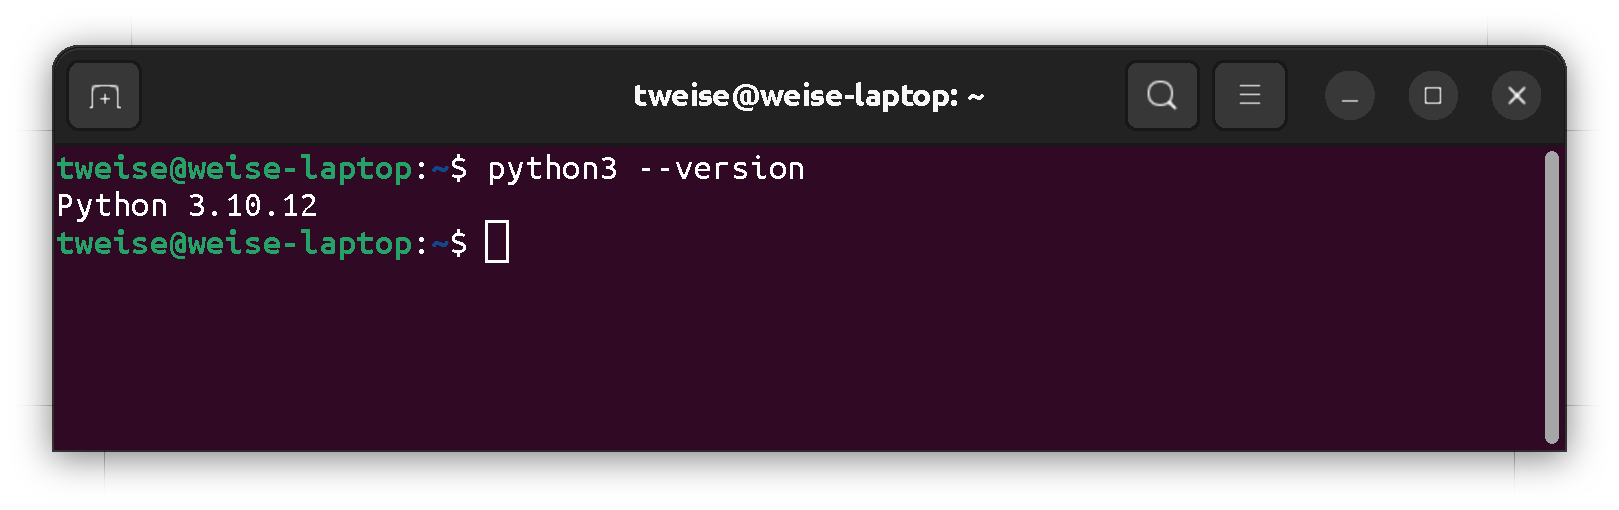
\includegraphics[width=0.7\linewidth]{\currentDir/ubuntuTerminalPythonVersion}%
\caption{Under \ubuntu\ \linux~\softwareStyle{22.04}, typing \bashil{python3 --version} in a \gls{terminal} and hitting return yields version~\softwareStyle{3.10}.}%
\label{fig:ubuntuTerminalPythonVersion}%
\end{figure}%
%
Under \ubuntu\ \linux, \python~\softwareStyle{3} is already pre-installed.
You can open a \gls{terminal}, type \bashil{python3 --version}, hit \keys{\return}, and get the result illustrated in \cref{fig:ubuntuTerminalPythonVersion}:%
My system has \python\ version~\softwareStyle{3.10} installed.%
%
\endhsection%
%
